\documentclass{beamer}
\usepackage{caption}
\usepackage{float}
\usepackage{lscape}
\usepackage{graphicx}% http://ctan.org/pkg/graphicx
\usepackage{booktabs}% http://ctan.org/pkg/booktabs
\usepackage{array}
\usepackage[export]{adjustbox}
\usepackage{amsmath}
\usepackage{amsfonts}
\usepackage{amssymb}
\usepackage{tikz}
\usepackage{ upgreek }
\usepackage{subcaption}
\usepackage{tabularx} 
\usepackage{setspace}
\usepackage{lipsum}
\usepackage{scalerel}


\graphicspath{ {images/} }
\usetheme{Frankfurt}
%\usefonttheme{structuresmallcapsserif} 
\definecolor{Gold}{RGB}{218,165,32}
\setbeamertemplate{navigation symbols}{}
\setbeamertemplate{theorems}[numbered]
\setbeamertemplate{theorems}[ams style] 
%\setbeamertemplate{navigation symbols}{}

\renewcommand{\qedsymbol}{$\blacksquare$}
\makeatletter

\setbeamerfont{footline}{size=\fontsize{6}{8.5}\selectfont}

\defbeamertemplate*{footline}{Dan P theme}
{
  \leavevmode%
  \hbox{%
  \begin{beamercolorbox}[wd=.15\paperwidth,ht=2.25ex,dp=1ex,center]{author in head/foot}%
    \usebeamerfont{author in head/foot}\insertshortauthor\expandafter\beamer@ifempty\expandafter{\beamer@shortinstitute}{}{~~(\insertshortinstitute)}
  \end{beamercolorbox}%
  \begin{beamercolorbox}[wd=.63\paperwidth,ht=2.25ex,dp=1ex,center]{title in head/foot}%
    \usebeamerfont{title in head/foot}\insertshorttitle
  \end{beamercolorbox}%
  \begin{beamercolorbox}[wd=.22\paperwidth,ht=2.25ex,dp=1ex,right]{date in head/foot}%
    \usebeamerfont{date in head/foot}\insertshortdate{}\hspace*{1.5em}
\insertframenumber{} / \inserttotalframenumber\hspace*{4ex} 
  \end{beamercolorbox}}%
  \vskip0pt%
}

\newcommand{\verysmallsize}{\@setfontsize{\srcsize}{5pt}{5pt}}

\makeatother

\title[Monetary Uncertainty as a Determinant of the Response of Stock Market to MNAs]{Monetary Uncertainty as a Determinant of the Response of Stock Market to Macroeconomic News Announcements\\ }

% many auto-annotations to stargazer tables are wrong, since 
% I usually copypasted tabular output into table environment
% from Nov 19 version.

\author{Mykola Pinchuk}

\date{03/15/2023}

\subject{Empirical Asset Pricing}



\newcommand\Wider[2][3em]{%
\makebox[\linewidth][c]{%
  \begin{minipage}{\dimexpr\textwidth+#1\relax}
  \raggedright#2
  \end{minipage}%
  }%
}


\begin{document}

\begin{frame}
  \titlepage
\end{frame}

\section{Overview}
\subsection{}


\begin{frame}{Introduction}
\begin{itemize}
    \item {\textbf{The Question: How does macroeconomic environment affect asset prices?}}
    \item {Macroeconomic News Announcements (MNA) provide perfect framework to answer the question.}    
    \item {Traditional approach uses low frequency analysis.}    
    \item {Using high-frequency event study of MNA has advantages:}
    \begin{itemize}
        \item {Higher signal-to-noise ratio.}
        \item {Higher statistical power.}
        \item {Ability to distinguish between effects of correlated macroeconomic variables.}
        \item {Causal interpretation of the results.}
    \end{itemize}
\end{itemize}
\end{frame}


\begin{frame}{Literature}
\begin{itemize}
    \item {Response of asset prices to macroeconomic news announcements (MNA):}
    \begin{itemize}
        \item {Schwert (1981), Pearce and Roley (1985), Cutler, Poterba and Summers (1988), \textbf{Roley and McQueen (1993)}, \textbf{Flannery and Protopapadakis (2002)}, \textbf{Boyd, Hu and Jagannathan (2005)}, Andersen, Bollerslev, Diebold and Vega (2007), Law, Song and Yaron (2021).}
    \end{itemize}
    \item {RM93 and BHJ05 argue that on average stocks respond negatively to MNA surprise.}
    \item {FP02 finds that there is no significant response on average.}
    \item {These findings are puzzling.}
\end{itemize}
\end{frame}


\begin{frame}{Main results}
\begin{itemize}
    \item {Stocks exhibit strong positive response to MNA surprise.}    
    \item {Response is highly time-varying and is stronger when monetary uncertainty is low.}    
    \item {There is large positive cash flow channel and time-varying negative risk-free rate channel.}
    \item {Prior research found negative stock response to MNA surprise due to very high monetary uncertainty in 1980s.}
    \item {MNA do not appear to have significant effect on risk premium.}
    \begin{itemize}
    \end{itemize}
\end{itemize}
\end{frame}

\section{Data and Basic Results}
\subsection{}



\begin{frame}{Data: Macroeconomic News Announcements (MNA)}
\begin{itemize}
    \item {17 types of MNA, released at monthly frequency, 1997-2019, Bloomberg.}
    \item {Investors' surveys for each MNA from Bloomberg.}
    \item {MNA surprise = Announced value - Mean expected value.}
    \item {To identify relevant news, I consider only MNA, which significantly affect volatility of market returns within 30-minutes window.}
    \item {5 relevant news:}
    \begin{itemize}
    \footnotesize
        \item {Nonfarm payroll (NFP)}
        \item {ISM Manufacturing (PMI)}
        \item {Retail Sales}
        \item {Consumer Confidence}
        \item {Construction Spending}
    \end{itemize}
    \item {I use intraday and daily asset prices to measure their response to MNA surprise.}
\end{itemize}
\end{frame}

\normalsize


\begin{frame}{Stock Response}
\begin{itemize}
    \item {$R_t = a + b Surprise_t + \epsilon_t.$}
\end{itemize}

\centering
\begin{table}[!htbp] \centering 
  \caption{Response of S\&P500 to MNA} 
  \label{}
\begin{tabular}{@{\extracolsep{5pt}} llll} 
\\[-1.8ex]\hline 
\hline \\[-1.8ex] 
Event & b & T-statistic(b) & R^2 \\ 
\hline \\[-1.8ex] 
Change in Nonfarm Payrolls & $0.25$ & $7.82$ & $0.20$ \\ 
ISM Manufacturing & $0.16$ & $5.20$ & $0.09$ \\ 
Conf. Board Consumer Confidence & $0.11$ & $4.87$ & $0.09$ \\ 
Retail Sales Advance MoM & $0.11$ & $5.87$ & $0.12$ \\ 
Construction Spending MoM & $0.07$ & $2.44$ & $0.02$ \\ 
Unemployment Rate & $0.06$ & $1.60$ & $0.01$ \\ 
\hline \\[-1.8ex] 
\end{tabular} 
\end{table} 

\end{frame}


\begin{frame}{Response in subsamples}
\begin{itemize}
    \item {$R_t = a + b Surprise_t + \epsilon_t.$}
\end{itemize}

\small
% Table created by stargazer v.5.2.2 by Marek Hlavac, Harvard University. E-mail: hlavac at fas.harvard.edu
% Date and time: Fri, Apr 09, 2021 - 2:33:57 PM
\begin{table}[!htbp] \centering 
  \label{} 
\begin{tabular}{@{\extracolsep{5pt}}lcccc} 
\\[-1.8ex]\hline 
\hline \\[-1.8ex] 
 & \multicolumn{4}{c}{\textit{Dependent variable:}} \\ 
\cline{2-5} 
\\[-1.8ex] & \multicolumn{4}{c}{SPX} \\ 
\\[-1.8ex] & (1) & (2) & (3) & (4)\\ 
\hline \\[-1.8ex] 
 Surprise & 0.203$^{***}$ & 0.141$^{***}$ & 0.244$^{***}$ & 0.094$^{***}$ \\ 
  & [4.552] & [9.998] & [12.869] & [4.987] \\ 
  & & & & \\ 
 Constant & $-$0.030 & 0.013 & 0.006 & 0.004 \\ 
  & [$-$0.444] & [1.014] & [0.384] & [0.206] \\ 
  & & & & \\ 
\hline \\[-1.8ex] 
Subsample & Recession & Expansion & Low MU & High MU \\ 
Observations & 96 & 891 & 514 & 473 \\ 
Adjusted R$^{2}$ & 0.172 & 0.100 & 0.243 & 0.048 \\ 
\hline 
\hline \\[-1.8ex] 
\end{tabular} 
\end{table} 
\end{frame}


\begin{frame}{Monetary uncertainty (MU)}
\begin{itemize}
    \item {I use implied volatility of 2-year Treasury rate to proxy for MU.}
    \item {Over the sample period, monetary uncertainty fluctuates between 0.2\% and 1.2\%.}
\end{itemize}
\centering
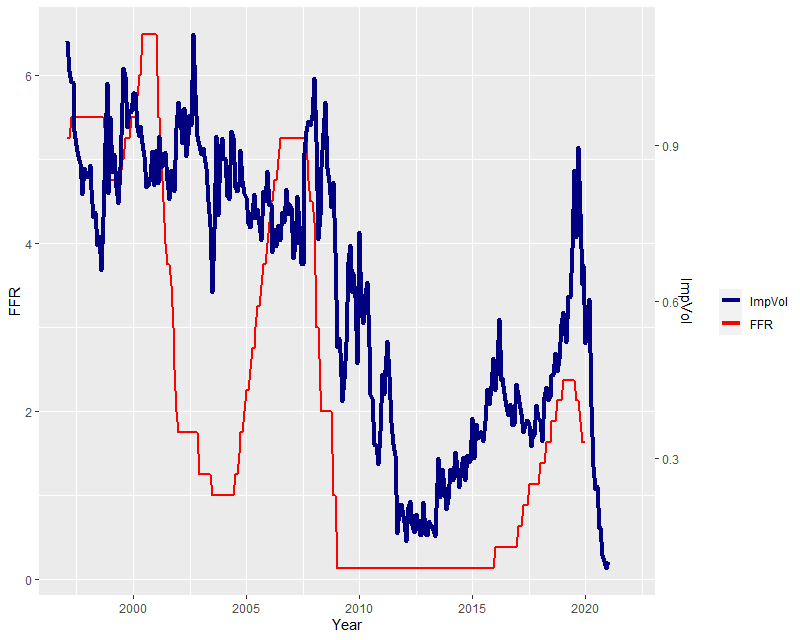
\includegraphics[width=0.64\textwidth]{images/imvol_ffr_plot.png}
\end{frame}



\section{Intuition \& Model}
\subsection{}

\begin{frame}{Why does monetary uncertainty vary?}
The Fed has time-varying ability and willingness to use its tools due to:
\begin{enumerate}
    \item Interest rate level
    \item Manner in which Fed Board conducts monetary policy (transparency, clarity, policy errors)
    \item Public debt level
\end{enumerate}
\end{frame}



\begin{frame}{Monetary uncertainty: ZLB}
    \begin{itemize}
        \item Monetary uncertainty varies with a level of short-term interest rate
        \item During a period of zero lower bound (ZLB) the Fed cannot cut rates
        \item Low interest rate means low monetary uncertainty
    \end{itemize}  
\end{frame}


\begin{frame}{Monetary uncertainty: Monetary policy implementation manner}
    \begin{itemize}
        \item In implementing monetary policy, the Fed balances its flexibility and policy transparency/continuity
        \item Volcker and Greenspan maintained minimum communication policy to maximize Fed flexibility
        \item Bernanke, Yellen and Powell (before 2022?) prioritized detailed communication over policy flexibility
        \item Clear and transparent monetary policy implies low monetary uncertainty
        \item Monetary uncertainty is elevated after Fed policy errors 
    \end{itemize}  
\end{frame}





\begin{frame}{Theoretical framework: Stock response}
    \begin{itemize}
    \abovedisplayskip=-\baselineskip
    \belowdisplayskip=0pt
    \abovedisplayshortskip=-\baselineskip
    \belowdisplayshortskip=0pt
        \item {$P = \frac{\mathbb{E}[D]}{R^F + RP}.$}
        \item {Assume MNA surprise is a pure growth shock $\epsilon_t$.}
        \item {Good MNA surprise affects stocks through higher expected cash flows and through higher expected risk-free rate.}
        \item 
        \begin{align}
        R_t = a_1 \epsilon_{t} + a_2 \Delta i_t + e_{1,t}.
        \end{align}
        \item 
        \begin{align}
        \Delta i_t = (\gamma_0 + \gamma_1 MU_{t-1})\epsilon_{t}+e_{2,t}.
        \end{align}
        \item 
        \begin{align}
        R_t = [a_1+a_2\gamma_0] \epsilon_{t} + [a_2 \gamma_1] MU_{t-1}\epsilon_{t} + e_{3,t}.
        \end{align}
        \item{Assumptions:}
        \begin{enumerate}
            \item {Risk premium is unaffected.}
            \item {Strength of cash flow channel does not depend on the monetary uncertainty MU.}
        \end{enumerate}
    \end{itemize}
\end{frame}


\begin{frame}{Intuition}
\begin{itemize}
    \item {Good MNA affects stocks through 2 channels:}
    \begin{enumerate}
        \item {Positive: Higher cash flow growth $\implies$ higher price.}
        \item {Negative: Higher probability of increasing rates $\implies$ lower price:}
        \begin{itemize}
                \item {Fed has dual mandate: full employment and price stability.}
                \item {Fed changes interest rates in response to changes in economic environment.}
        \end{itemize}
    \end{enumerate}
    \item {Strength of monetary channel varies over time:}
    \begin{itemize}
    \item {Monetary channel is small when monetary uncertainty is low.}
    \item {Zero monetary uncertainty allows us to shut down risk-free channel.}
    \end{itemize}
\end{itemize}
\end{frame}


\section{Decomposition}
\subsection{}


\begin{frame}{Results: Regression with interaction term, interest rates}{$\Delta i_t = c_0*Surprise_t + c_1*MU_{t-1} + c_2*Surprise_t*MU_{t-1} + e_t$}
%\vskip -0.1
\vspace{-0.1cm}
\centering
%\vskip -0.1
\vstretch{0.88}{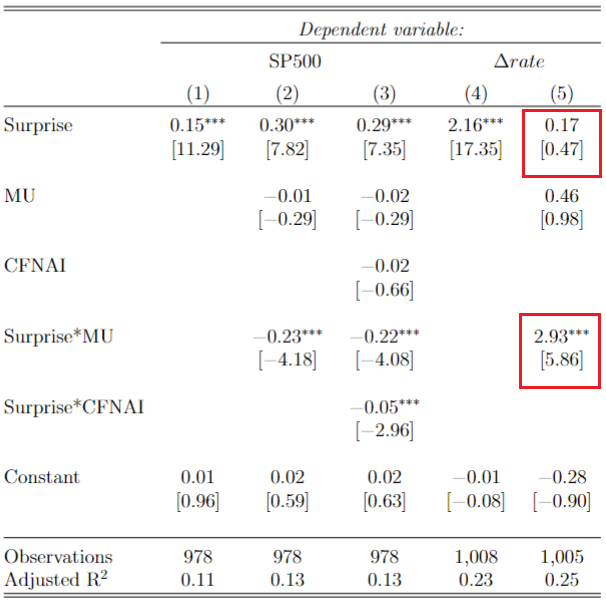
\includegraphics[width=0.78\textwidth]{images/dp_f7bon.png}}   
\end{frame}



\begin{frame}{Results: Regression with interaction term, stocks}
{$R_t = b*Surprise_t + c*MU_{t-1} + d*Surprise_t*MU_{t-1} + e_t$}
\vspace{-0.3cm}
\centering
\vspace{0.2cm}
\vstretch{0.88}{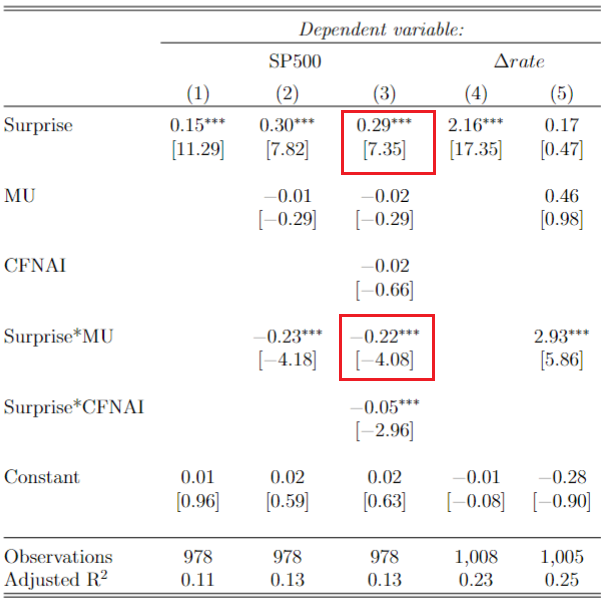
\includegraphics[width=0.78\textwidth]{images/dp_f7st.png}}   
\small
\end{frame}


\begin{frame}{Results: Coefficient estimates}
\centering
\vspace{0.2cm}
\begin{itemize}
        \item {$\Delta i_t = (\gamma_1 MU_{t-1})\epsilon_{t}+e_{2,t}.$}
        \item 
        \begin{aligned*}
            R_t = \underbrace{a_1 \epsilon_{t}}_{\substack{\text{Cash flow}\\\text{channel}}} + \underbrace{a_2 \Delta i_t}_{\substack{\text{Risk-free rate}\\\text{channel}}} + e_{1,t}.
        \end{aligned*}
        %\underbrace{\rho T\dfrac{D s}{D t}}_{\substack{\text{Entropy}\\\text{advection}}} = 
        \item {$R_t = [a_1] \epsilon_{t} + [a_2 \gamma_1] MU_{t-1}\epsilon_{t}.$}
        \vspace{0.4cm}
        \item{Estimates:}
        \begin{itemize}
            \item {$\gamma_1 = 2.9 \ bps$.}
            \item {$a_1 = 30 \ bps$.}
            \item {$a_2 = -8$.}
        \end{itemize}
        \item {1 $\sigma$ of good news leads to 30 bps returns through cash flow channel.}
        \item {1 $\sigma$ of good news leads to -23 bps returns per 1\% monetary uncertainty through monetary channel.}
\end{itemize}
\end{frame}


\normalsize

\section{Other Results}
\subsection{}


\begin{frame}{Extrapolating results to earlier sample}
\begin{itemize}
    \item {I have the data over 1997-2019, hence cannot decompose the response in the earlier sample.}
    \item {To extrapolate my results to the period before 1997, I need different proxy for monetary uncertainty.}
    \item {I use realized volatility of 2-year T-note over 2 years.}
\end{itemize}
\end{frame}



\small
\begin{frame}{Decomposition, regression with interaction term}
{$R_t = b*Surprise_t + c*Vol^{TN2}_{t-1} + d*Surprise_t*Vol^{TN2}_{t-1} + e_t$}
% Table created by stargazer v.5.2.3 by Marek Hlavac, Social Policy Institute. E-mail: marek.hlavac at gmail.com
% Date and time: Sun, Sep 18, 2022 - 1:56:10 PM
\begin{table}[!htbp] \centering 
{\renewcommand{\arraystretch}{0.88}
\begin{tabular}{@{\extracolsep{5pt}}lcc} 
\\[-1.8ex]\hline 
\hline \\[-1.8ex] 
 & \multicolumn{2}{c}{\textit{Dependent variable:}} \\ 
\cline{2-3} 
\\[-1.8ex] & \multicolumn{2}{c}{SPX} \\ 
\\[-1.8ex] & (1) & (2)\\ 
\hline \\[-1.8ex] 
 Surprise & 0.15$^{***}$ & 0.20$^{***}$ \\ 
  & [11.29] & [7.95] \\ 
  & & \\ 
 Vol^{TN2} &  & $-$0.003 \\ 
  &  & [$-$0.04] \\ 
  & & \\ 
 Surprise*Vol^{TN2} &  & $-$0.16$^{***}$ \\ 
  &  & [$-$2.94] \\ 
  & & \\ 
 Constant & 0.01 & 0.01 \\ 
  & [0.96] & [0.65] \\ 
  & & \\ 
\hline \\[-1.8ex] 
Observations & 978 & 978 \\ 
Adjusted R$^{2}$ & 0.11 & 0.13 \\ 
\hline 
\hline \\[-1.8ex] 
\end{tabular}}
\end{table}
\end{frame}



\normalsize
\begin{frame}{Response of stocks to 1 sigma MNA shock}
\centering
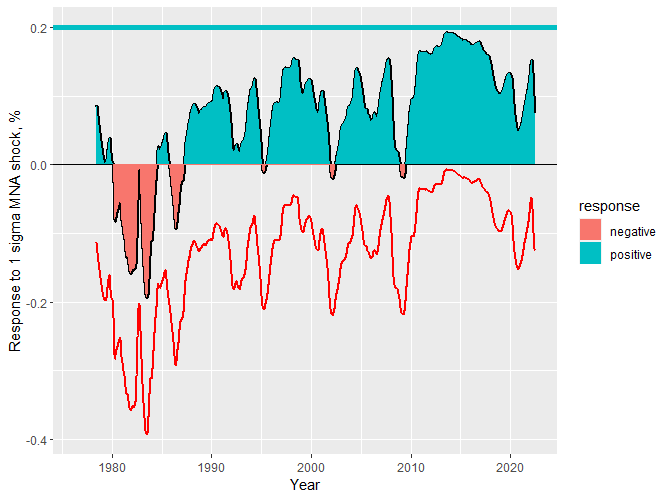
\includegraphics[width=0.94\textwidth]{images/1980s_plot2.png}
\end{frame}



\begin{frame}{Different maturities}
\begin{columns}
\begin{column}{0.6\textwidth}
\vstretch{0.9}{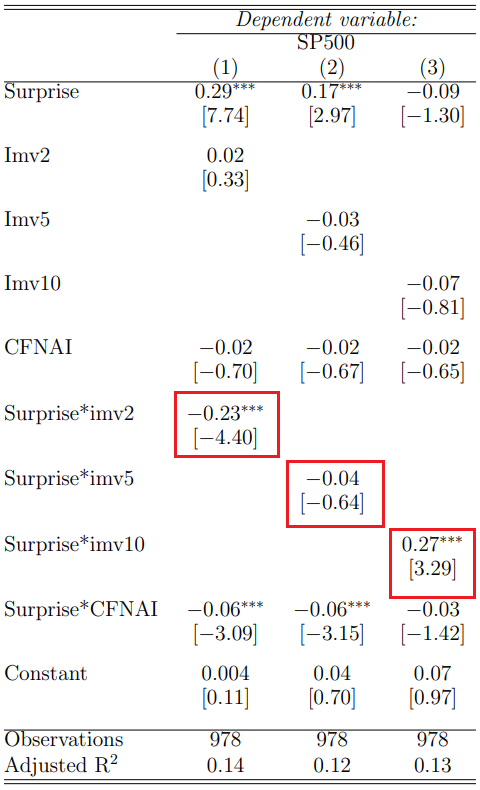
\includegraphics[width=0.8\textwidth]{images/dp_t11.png}}
\end{column}
\begin{column}{0.5\textwidth}  %%<--- here
\begin{itemize}
    \item When implied volatility of 2-year rate is high, negative channel is stronger.
    \vspace{0.5cm}
    \item When implied volatility of 10-year rate is high, positive channel is stronger.
\end{itemize}
\end{column}
\end{columns}    
\end{frame}


\begin{frame}{Macroeconomic Uncertainty}
\centering
\vspace{-0.1cm}
\vstretch{0.88}{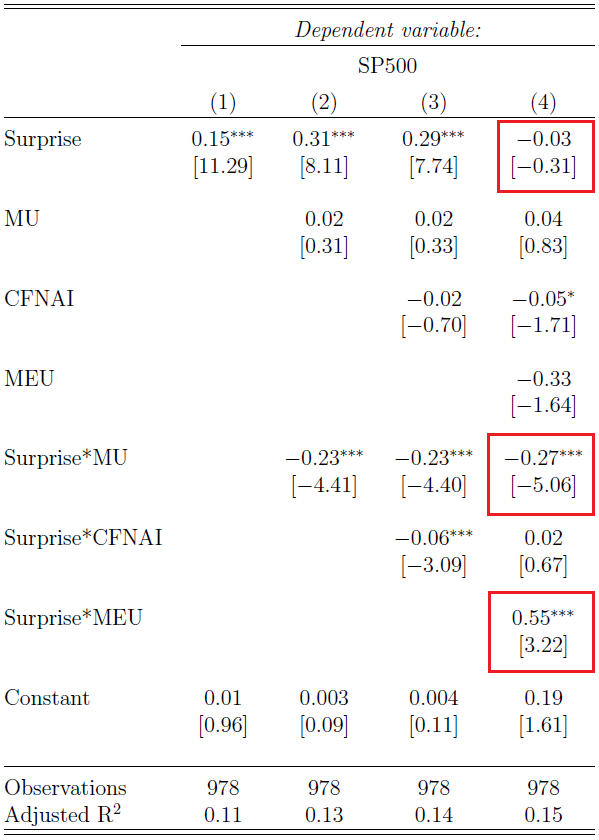
\includegraphics[width=0.59\textwidth]{images/dp_f9.png}}   
\end{frame}


\section{Cross-section}
\subsection{}

\begin{frame}{Cross-Sectional Results}
\begin{itemize}
    \item {We can test whether these MNA are priced in cross-section of expected stock returns.}
    \item {For each stock and MNA, estimate $\beta_i^{MNA}$ and see whether long-short portfolio on $\beta^{MNA}$ produces significant returns.}
    \item {$R_t = \alpha + \beta^{MNA}* surprise_t^{MNA}+e_t$.}
    \item {I use 4-year rolling window to estimate $\beta^{MNA}$ for each MNA type.}
    \item {I divide stocks into quintile portfolios on $\beta^{MNA}$ and estimate their returns.}
\end{itemize}
\end{frame}



\begin{frame}{Average returns of quintile portfolios, sorted on $\beta^{MNA}$}
\centering
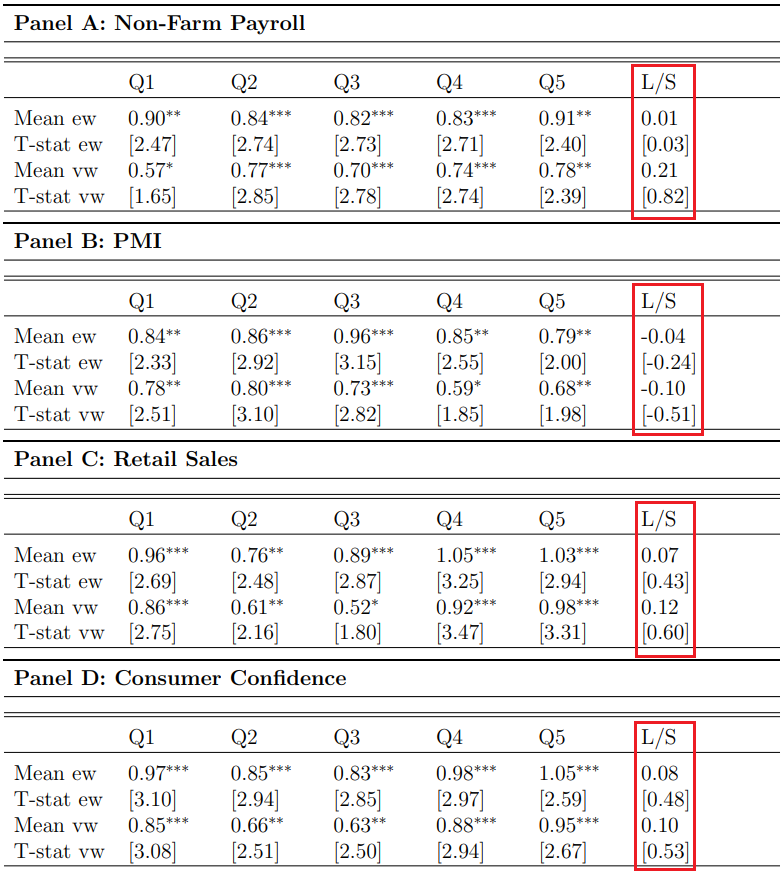
\includegraphics[width=0.64\textwidth]{images/dp_t13.png}  
\end{frame}


\begin{frame}{Abnormal returns of quintile portfolios, sorted on $\beta_{MNA}$}
\centering
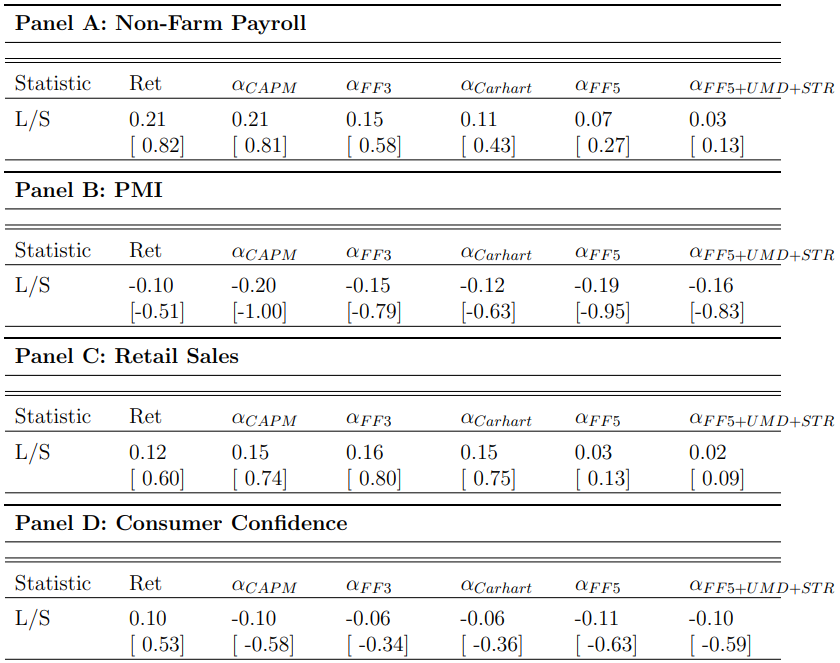
\includegraphics[width=0.85\textwidth]{images/dp_t14.png}  
\end{frame}



\section{Conclusion}
\subsection{}

\begin{frame}{Conclusion}
\Wider[2em]{
\begin{itemize}
    \item {Stocks exhibit strong positive response (10-25 bps) to MNA surprise.}    
    \item {The response is highly time-varying and is stronger when monetary uncertainty is low.}    
    \item {There is large positive cash flow channel (30 bps) and time-varying negative risk-free rate channel (-23 bps when monetary uncertainty is 1\%).}
    \item {Prior research found negative stock response to MNA surprise. I explain in by very high monetary uncertainty in the 1980s.}
    \item {Overall, monetary policy is crucial to understand this response. }
\end{itemize}}
\end{frame}


\section{Appendix}
\subsection{}


\begin{frame}{Response of T-notes to MNA surprise, more controls}
\begin{table}[!htbp] 
    \centering 
    \tiny 
{\renewcommand{\arraystretch}{0.84}
\begin{tabular}{@{\extracolsep{5pt}}lccccc} 
\\[-1.8ex]\hline 
\hline \\[-1.8ex] 
 & \multicolumn{5}{c}{\textit{Dependent variable: $\Delta i_2$}} \\ 
\cline{2-6} 
\\[-1.8ex] & (1) & (2) & (3) & (4) & (5)\\ 
\hline \\[-1.8ex] 
 Surprise & 2.16$^{***}$ & 0.26 & $-$0.03 & 0.02 & 0.56 \\ 
  & [17.35] & [0.74] & [$-$0.09] & [0.04] & [1.13] \\ 
  & & & & & \\ 
 Surprise*MU &  & 2.76$^{***}$ & 3.86$^{***}$ & 4.00$^{***}$ & 4.08$^{***}$ \\
  &  & [5.72] & [6.39] & [6.16] & [6.20] \\ 
  & & & & & \\ 
 Surprise*FFR &  &  & $-$0.21$^{**}$ &  &  \\ 
  &  &  & [$-$2.57] &  &  \\ 
  & & & & & \\ 
 Surprise*TN2 &  &  &  & $-$0.23$^{**}$ &  \\ 
  &  &  &  & [$-$2.42] &  \\ 
  & & & & & \\ 
 Surprise*CFNAI &  &  &  &  & 0.59$^{**}$ \\ 
  &  &  &  &  & [2.21] \\ 
  & & & & & \\ 
 Surprise*VIX &  &  &  &  & $-$0.04$^{**}$ \\ 
  &  &  &  &  & [$-$2.31] \\ 
  & & & & & \\ 
 Surprise*P/D &  &  &  &  & $-$0.26$^{*}$ \\ 
  &  &  &  &  & [$-$1.76] \\ 
  & & & & & \\ 
 Surprise*Infl &  &  &  &  & $-$0.23$^{*}$ \\ 
  &  &  &  &  & [$-$1.91] \\ 
  & & & & & \\ 
 Constant & $-$0.01 & $-$0.68$^{**}$ & $-$0.77$^{**}$ & $-$0.78$^{**}$ & $-$0.64 \\ 
  & [$-$0.08] & [$-$2.18] & [$-$2.34] & [$-$2.43] & [$-$1.40] \\ 
  & & & & & \\ 
\hline \\[-1.8ex] 
Observations & 1,008 & 1,005 & 1,001 & 1,001 & 963 \\ 
Adjusted R$^{2}$ & 0.23 & 0.26 & 0.27 & 0.27 & 0.28 \\ 
\hline 
\hline \\[-1.8ex] 
\end{tabular}  
}
\end{table}
\end{frame}



\begin{frame}{Response of stocks to MNA surprise, more controls}
\begin{table}[!htbp] 
\centering 
\scriptsize
\begin{tabular}{@{\extracolsep{5pt}}lcccc} 
\\[-1.8ex]\hline 
\hline \\[-1.8ex] 
 & \multicolumn{4}{c}{\textit{Dependent variable:}} \\ 
\cline{2-5} 
\\[-1.8ex] & \multicolumn{4}{c}{SP500} \\ 
\\[-1.8ex] & (1) & (2) & (3) & (4)\\ 
\hline \\[-1.8ex] 
 Surprise & 0.16$^{***}$ & 0.30$^{***}$ & 0.29$^{***}$ & 0.17$^{***}$ \\ 
  & [11.48] & [7.83] & [7.43] & [3.31] \\ 
  & & & & \\ 
 Surprise*MU &  & $-$0.21$^{***}$ & $-$0.21$^{***}$ & $-$0.25$^{***}$ \\ 
  &  & [$-$4.05] & [$-$4.04] & [$-$4.34] \\ 
  & & & & \\ 
 Surprise*CFNAI &  &  & $-$0.06$^{***}$ & 0.01 \\ 
  &  &  & [$-$3.25] & [0.49] \\ 
  & & & & \\ 
 Surprise*VIX &  &  &  & 0.01$^{***}$ \\ 
  &  &  &  & [3.50] \\ 
  & & & & \\ 
 Constant & 0.01 & 0.01 & 0.01 & $-$0.01 \\ 
  & [0.65] & [0.17] & [0.24] & [$-$0.24] \\ 
  & & & & \\ 
\hline \\[-1.8ex] 
Observations & 986 & 986 & 986 & 946 \\ 
Adjusted R$^{2}$ & 0.12 & 0.13 & 0.14 & 0.14 \\ 
\hline 
\hline \\[-1.8ex] 
\textit{Note:}  & \multicolumn{4}{r}{$^{*}$p$<$0.1; $^{**}$p$<$0.05; $^{***}$p$<$0.01} \\ 
\end{tabular} 
\end{table}
\end{frame}




\normalsize

\begin{frame}{Pre-ranking betas vs Post-ranking betas}
\centering
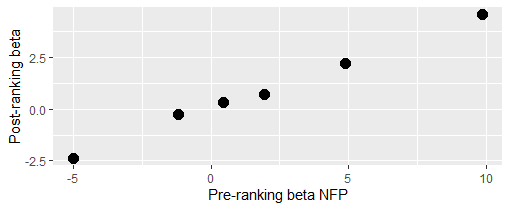
\includegraphics[width=0.85\textwidth]{old_files/i102_f1a.png}
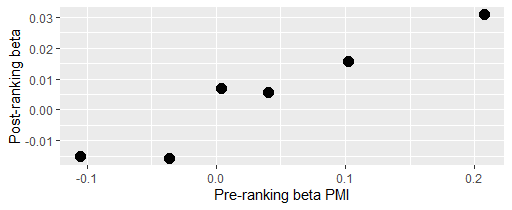
\includegraphics[width=0.85\textwidth]{old_files/i102_f1b.png}  
\end{frame}


\begin{frame}{More on RP channel:}
There may be two types of RP channels:
    \begin{itemize}
        \item {Positive: Good growth shock decreases RP (e.g., rare disaster model)}
        \item {Negative: Good growth shock raises RP. RP is an amplifier of a change in risk-free rate via RFY channel (Hanson and Stein 2015)}
    \end{itemize}
\vspace{0.3cm}
{There is no RP channel, which is consistent with all my results:}
\vspace{0.3cm}
\begin{tabular}{|p{42mm}|c|c|c|}
\hline
    Result \Channels & CF & Positive RP & Negative RP \\ 
\hline
    Stock response & Yes & Yes? & No\\ 
\hline
    Yield curve response & Yes & No & Yes\\ 
\hline
    Term premium response with an interaction term & N/A & No & No\\ 
\hline
    Cross-sectional spread & N/A & No & No\\ 
\hline
\end{tabular}
\end{frame}



\begin{frame}{Results: Term structure response}
\centering
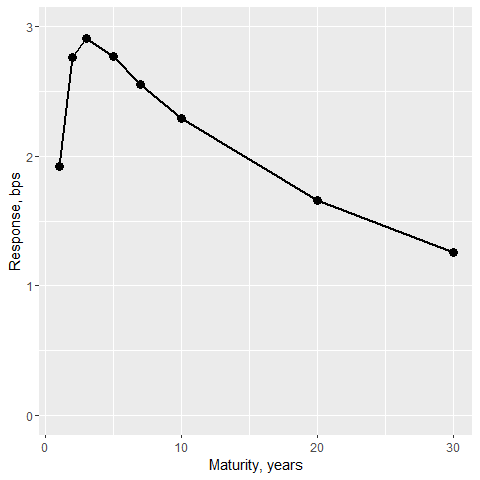
\includegraphics[width=0.72\textwidth]{old_files/F2_termstructure_0.png}
\end{frame}


\begin{frame}{Measurement accuracy}
\begin{itemize}
    \item {$R_t = a + b Surprise_t + \epsilon_t.$}
\end{itemize}
% Table created by stargazer v.5.2.2 by Marek Hlavac, Harvard University. E-mail: hlavac at fas.harvard.edu
% Date and time: Fri, Apr 09, 2021 - 2:09:45 PM
\begin{table}[!htbp] \centering 
{\renewcommand{\arraystretch}{0.9}
\begin{tabular}{@{\extracolsep{2pt}}lcccc} 
\\[-1.8ex]\hline 
\hline \\[-1.8ex] 
 & \multicolumn{4}{c}{\textit{Dependent variable:}} \\ 
\cline{2-5} 
\\[-1.8ex] & vwretd & SP500 & SP500 & SP500 \\ 
\\[-1.8ex] & (1) & (2) & (3) & (4)\\ 
\hline \\[-1.8ex] 
 PMI surprise & 0.160$^{**}$ & 0.169$^{**}$ & 0.193$^{***}$ & 0.156$^{***}$ \\ 
  & [1.994] & [2.027] & [3.142] & [5.135] \\ 
  & & & & \\ 
 Constant & 0.163$^{**}$ & 0.165$^{*}$ & 0.105$^{*}$ & $-$0.008 \\ 
  & [2.018] & [1.961] & [1.696] & [$-$0.260] \\ 
  & & & & \\ 
\hline \\[-1.8ex] 
Announcement window & Day & Day & Half-day & 30 minutes \\ 
Observations & 276 & 266 & 266 & 266 \\ 
Adjusted R$^{2}$ & 0.011 & 0.012 & 0.032 & 0.087 \\ 
\hline 
\hline \\[-1.8ex] 
\end{tabular}}
\end{table}
\end{frame}


\begin{frame}{Stock response over 2.5 hours}
\centering
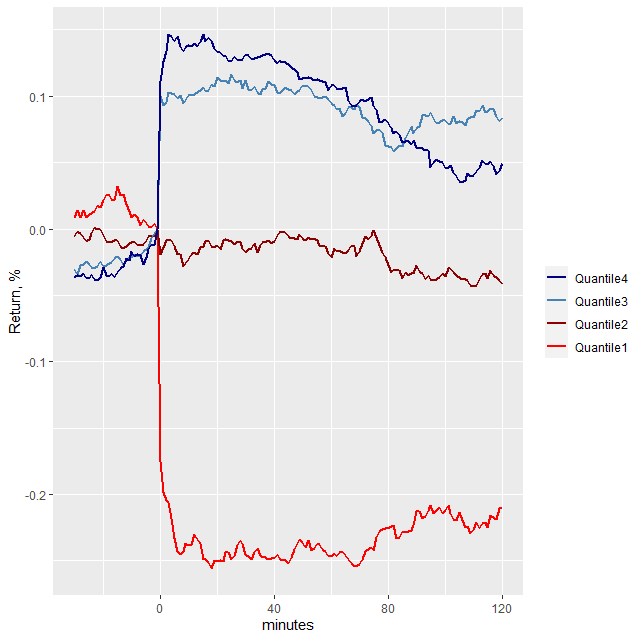
\includegraphics[width=0.72\textwidth]{images/hf_response.png}  
\end{frame}




\begin{frame}{Term Premium response}
\scriptsize
    % Table created by stargazer v.5.2.3 by Marek Hlavac, Social Policy Institute. E-mail: marek.hlavac at gmail.com
% Date and time: Mon, Nov 28, 2022 - 5:09:57 PM
\begin{table}[!htbp] \centering 
{\renewcommand{\arraystretch}{1}
\begin{tabular}{@{\extracolsep{5pt}}lcccc} 
\\[-1.8ex]\hline 
\hline \\[-1.8ex] 
 & \multicolumn{4}{c}{\textit{Dependent variable:}} \\ 
\cline{2-5} 
\\[-1.8ex] & \multicolumn{4}{c}{d\_TP^{10-2}} \\ 
\\[-1.8ex] & (1) & (2) & (3) & (4)\\ 
\hline \\[-1.8ex] 
 surprise & $-$0.31$^{***}$ & 1.90$^{***}$ & 1.91$^{***}$ & 2.48$^{***}$ \\ 
  & [$-$4.77] & [10.99] & [10.94] & [4.96] \\ 
  & & & & \\ 
 surprise:imv2 &  & $-$3.23$^{***}$ & $-$3.23$^{***}$ & $-$3.17$^{***}$ \\ 
  &  & [$-$13.61] & [$-$13.61] & [$-$13.00] \\ 
  & & & & \\ 
 surprise:CFNAI &  &  & 0.004 & $-$0.14 \\ 
  &  &  & [0.05] & [$-$0.99] \\ 
  & & & & \\ 
 surprise:MEU &  &  &  & $-$0.95 \\ 
  &  &  &  & [$-$1.21] \\ 
  & & & & \\ 
 Constant & $-$0.01 & 0.05 & 0.04 & $-$0.83 \\ 
  & [$-$0.14] & [0.31] & [0.25] & [$-$1.50] \\ 
  & & & & \\ 
\hline \\[-1.8ex] 
Observations & 1,008 & 1,005 & 1,005 & 1,005 \\ 
Adjusted R$^{2}$ & 0.02 & 0.17 & 0.17 & 0.17 \\ 
\hline 
\hline \\[-1.8ex] 
\end{tabular} }
\end{table}
\end{frame}





\scriptsize
\begin{frame}{Summary statistics of MNA}
\begin{table}[!htbp] \centering 
\begin{tabular}{@{\extracolsep{-6pt}} lllllllllllll} 
\\[-1.8ex]\hline 
\hline \\[-1.8ex] 
News & Variable & Min & p1 & p10 & p25 & Median & p75 & p90 & p99 & Max & Mean & SD \\ 
\hline \\[-1.8ex] 
All & CFNAI & $$-$3.35$ & $$-$2.68$ & $$-$0.61$ & $$-$0.31$ & $0.02$ & $0.28$ & $0.50$ & $0.94$ & $1.21$ & $$-$0.07$ & $0.60$ \\ 
All & USREC & $0$ & $0$ & $0$ & $0$ & $0$ & $0$ & $0$ & $1$ & $1$ & $0.09$ & $0.29$ \\ 
All & FFR_{t-1} & $0.12$ & $0.12$ & $0.12$ & $0.12$ & $1.62$ & $4.75$ & $5.50$ & $6.50$ & $6.50$ & $2.25$ & $2.14$ \\ 
All & drate & $$-$0.09$ & $$-$0.05$ & $$-$0.01$ & $0$ & $0$ & $0$ & $0.01$ & $0.04$ & $0.09$ & $0$ & $0.01$ \\ 
NFP & spx\_ret & $$-$2.03$ & $$-$1.46$ & $$-$0.66$ & $$-$0.20$ & $0.10$ & $0.31$ & $0.72$ & $1.41$ & $1.97$ & $0.04$ & $0.56$ \\ 
NFP & surprise & $$-$3.93$ & $$-$2.90$ & $$-$1.31$ & $$-$0.68$ & $$-$0.06$ & $0.44$ & $1.02$ & $2.19$ & $3.22$ & $$-$0.13$ & $1$ \\ 
PMI & spx\_ret & $$-$3.26$ & $$-$1.34$ & $$-$0.57$ & $$-$0.29$ & $0.01$ & $0.23$ & $0.50$ & $1.47$ & $2.17$ & $0$ & $0.52$ \\ 
PMI & surprise & $$-$3.23$ & $$-$2.45$ & $$-$1.13$ & $$-$0.59$ & $0$ & $0.66$ & $1.32$ & $2.37$ & $3.98$ & $0.06$ & $1$ \\ 
Retail & spx\_ret & $$-$1.49$ & $$-$0.93$ & $$-$0.30$ & $$-$0.08$ & $0.02$ & $0.16$ & $0.33$ & $0.93$ & $1.04$ & $0.02$ & $0.32$ \\ 
Retail & surprise & $$-$3$ & $$-$2.62$ & $$-$0.94$ & $$-$0.56$ & $0$ & $0.37$ & $0.94$ & $2.68$ & $8.62$ & $$-$0.02$ & $1$ \\ 
Constr & spx\_ret & $$-$3.26$ & $$-$1.23$ & $$-$0.47$ & $$-$0.24$ & $0.03$ & $0.22$ & $0.50$ & $1.45$ & $2.17$ & $0.02$ & $0.50$ \\ 
Constr & surprise & $$-$7.71$ & $$-$2.18$ & $$-$1.09$ & $$-$0.51$ & $0$ & $0.45$ & $0.86$ & $2.17$ & $4.20$ & $$-$0.06$ & $1$ \\ 
Unempl & spx\_ret & $$-$2.03$ & $$-$1.46$ & $$-$0.66$ & $$-$0.20$ & $0.10$ & $0.31$ & $0.72$ & $1.41$ & $1.97$ & $0.04$ & $0.56$ \\ 
Unempl & surprise & $$-$3.52$ & $$-$2.34$ & $$-$1.41$ & $$-$0.70$ & $0$ & $0.70$ & $0.70$ & $2.11$ & $2.81$ & $$-$0.18$ & $1$ \\ 
CPI & spx\_ret & $$-$1.87$ & $$-$0.95$ & $$-$0.31$ & $$-$0.11$ & $0.02$ & $0.13$ & $0.35$ & $0.80$ & $2.47$ & $0.01$ & $0.35$ \\ 
CPI & surprise & $$-$3.35$ & $$-$2.52$ & $$-$0.84$ & $$-$0.84$ & $0$ & $0.84$ & $0.84$ & $2.52$ & $3.35$ & $$-$0.06$ & $1.01$ \\ 
PPI & spx\_ret & $$-$1.43$ & $$-$0.80$ & $$-$0.30$ & $$-$0.12$ & $$-$0.01$ & $0.12$ & $0.27$ & $0.84$ & $0.97$ & $$-$0.01$ & $0.29$ \\ 
PPI & surprise & $$-$2.91$ & $$-$2.91$ & $$-$0.97$ & $$-$0.48$ & $0$ & $0.48$ & $1.19$ & $2.76$ & $4.12$ & $0.02$ & $1$ \\ 
\hline \\[-1.8ex] 
\end{tabular} 
\end{table}
\end{frame}

\begin{frame}{Absolute returns during MNA}
\begin{table}[!htbp] \centering 
\begin{tabular}{@{\extracolsep{2pt}} lllll} 
\\[-1.8ex]\hline 
\hline \\[-1.8ex] 
News & Mean & Median & p-value (t) & p-value (MWW) \\ 
\hline \\[-1.8ex] 
Non-Farm Payroll & $0.41$ & $0.29$ & $0$ & $0$ \\ 
ISM Manufacturing & $0.36$ & $0.27$ & $0.0000$ & $0$ \\ 
Retail Sales Advance MoM & $0.21$ & $0.13$ & $0.0000$ & $0$ \\ 
Construction Spending MoM & $0.34$ & $0.23$ & $0.0000$ & $0$ \\ 
CPI MoM & $0.21$ & $0.13$ & $0.0001$ & $0$ \\ 
PPI MoM & $0.19$ & $0.12$ & $0.0002$ & $0$ \\ 
Conf. Board Consumer Confidence & $0.29$ & $0.18$ & $0.03$ & $0.12$ \\ 
Capacity Utilization & $0.17$ & $0.10$ & $0.14$ & $0.37$ \\ 
U. of Mich. Sentiment F & $0.27$ & $0.18$ & $0.28$ & $0.17$ \\ 
Trade Balance & $0.16$ & $0.10$ & $0.31$ & $0.03$ \\ 
Business Inventories & $0.23$ & $0.16$ & $0.40$ & $0.53$ \\ 
Housing Starts & $0.15$ & $0.09$ & $0.40$ & $0.07$ \\ 
Factory Orders & $0.24$ & $0.17$ & $0.46$ & $0.97$ \\ 
Leading Index & $0.26$ & $0.19$ & $0.47$ & $0.29$ \\ 
U. of Mich. Sentiment P & $0.26$ & $0.16$ & $0.76$ & $0.66$ \\ 
Monthly Budget Statement & $0.17$ & $0.11$ & $0.78$ & $0.33$ \\ 
New Home Sales & $0.25$ & $0.16$ & $0.79$ & $0.86$ \\ 
Durable Goods Orders & $0.14$ & $0.09$ & $0.84$ & $0.17$ \\ 
Consumer Credit & $0.20$ & $0.12$ & $0.91$ & $0.66$ \\ 
\hline \\[-1.8ex] 
\end{tabular} 
\end{table}
\end{frame}

\begin{frame}{Term structure response to MNA surprise}
\begin{table}[!htbp] \centering 
  \caption{\textbf{Interest rate response to major MNA}} 
  \label{}
\begin{tabular}{@{\extracolsep{-4pt}}lcccccccc} 
\\[-1.8ex]\hline 
\hline \\[-1.8ex] 
 & \multicolumn{8}{c}{\textit{Dependent variable:}} \\ 
\cline{2-9} 
\\[-1.8ex] & \Delta i_1 & \Delta i_2 & \Delta i_3 & \Delta i_5 & \Delta i_7 & \Delta i_{10} & \Delta i_{20} & \Delta i_{30} \\ 
\\[-1.8ex] & (1) & (2) & (3) & (4) & (5) & (6) & (7) & (8)\\ 
\hline \\[-1.8ex] 
 Surprise & 1.92$^{***}$ & 2.77$^{***}$ & 2.91$^{***}$ & 2.77$^{***}$ & 2.56$^{***}$ & 2.29$^{***}$ & 1.66$^{***}$ & 1.26$^{***}$ \\ 
  & [9.42] & [9.85] & [9.92] & [9.16] & [8.78] & [8.47] & [7.62] & [7.09] \\ 
  & & & & & & & & \\ 
 Constant & $-$0.07 & $-$0.07 & 0.10 & 0.31 & 0.39 & 0.37 & 0.25 & 0.19 \\ 
  & [$-$0.30] & [$-$0.24] & [0.31] & [0.91] & [1.20] & [1.24] & [1.05] & [0.94] \\ 
  & & & & & & & & \\ 
\hline \\[-1.8ex] 
Observations & 491 & 491 & 491 & 491 & 491 & 491 & 491 & 491 \\ 
Adjusted R$^{2}$ & 0.15 & 0.16 & 0.17 & 0.14 & 0.13 & 0.13 & 0.10 & 0.09 \\ 
\hline 
\hline \\[-1.8ex] 
\end{tabular} 
\end{table}
\end{frame}


\normalsize
\begin{frame}{Duration effect}
\begin{itemize}
    \item High interest rate implies lower duration. 
    \item "Duration" is $\hat{a}_2=-8$.
    \item High monetary uncertainty mechanically produces smaller duration, hence lower estimate of risk-free channel (assuming fixed coefficients for bond response).
    \item Thus the estimate of the monetary channel is the lower bound (in absolute value) of this channel. 
\end{itemize}
\end{frame}




\end{document}

